\documentclass{article}
\usepackage[UTF8]{ctex}
\usepackage{geometry}
\usepackage{natbib}
\geometry{left=3.18cm,right=3.18cm,top=2.54cm,bottom=2.54cm}
\usepackage{graphicx}
\pagestyle{plain}	
\usepackage{setspace}
\usepackage{caption2}
\usepackage{datetime} %日期
\renewcommand{\today}{\number\year 年 \number\month 月 \number\day 日}
\renewcommand{\captionlabelfont}{\small}
\renewcommand{\captionfont}{\small}
\begin{document}

\begin{figure}
    \centering
    
\includegraphics[width=8cm]{upc.png}

    \label{figupc}
\end{figure}

	\begin{center}
		\quad \\
		\quad \\
		\heiti \fontsize{45}{17} \quad \quad \quad 
		\vskip 1.5cm
		\heiti \zihao{2} 《计算科学导论》课程总结报告
	\end{center}
	\vskip 2.0cm
		
	\begin{quotation}
% 	\begin{center}
		\doublespacing
		
        \zihao{4}\par\setlength\parindent{7em}
		\quad 

		学生姓名:\underline{\qquad  曹双 \qquad \qquad}

		学\hspace{0.61cm} 号:\underline{\qquad 1907010111\qquad}
		
		专业班级:\underline{\qquad 计算1901 \qquad  }
		
        学\hspace{0.61cm} 院:\underline{计算机科学与技术学院}
% 	\end{center}
		\vskip 2cm
		\centering
		\begin{table}[h]
            \centering 
            \zihao{4}
            \begin{tabular}{|c|c|c|c|c|c|c|}
            % 这里的rl 与表格对应可以看到,姓名是r,右对齐的;学号是l,左对齐的;若想居中,使用c关键字。
                \hline
                课程认识 & 问题思 考 & 格式规范  & IT工具  & Latex附加  & 总分 & 评阅教师 \\
                30\% & 30\% & 20\% & 20\% & 10\% &  &  \\
                \hline
                 & & & & & &\\
                & & & & & &\\
                \hline
            \end{tabular}
        \end{table}
		\vskip 2cm
		\today
	\end{quotation}

\thispagestyle{empty}
\newpage
\setcounter{page}{1}
% 在这之前是封面,在这之后是正文
\section{引言}
计算科学导论这门课程,是计算机科学与技术的基础必修课,是针对计算机科学初学者而开设的铺垫性学科。导论的目的是站在科学的角度用高级科普的知识向读者提供一个了解和学习有关计算机专业的知识,包括历史、概念、意义、内容和方法等计算科学方面的系统知识,从而引导学生怎么从科学哲学的角度去认识和学习计算科学。这些内容对学生学好计算科学、顺利完成学业是有益的。这门课程并不强调对书中的主要内容掌握的熟练程度,但要求我们对计算机科学有一个较为完整的知识体系,个人认为这才是我们大一学生学习计算科学导论的意义所在。\par
我作为一名计算机科学与技术的大一学生,很荣幸听到孙运雷教授为我们讲授精彩丰富的计算科学导论课程。孙教授带领我们19级全体计算机科学与技术专业的七十多名同学与本研一体化班的同学们领略到了计算机这一当下十分热门专业的许多知识,开拓了我们的视野,丰富了我们的知识,孙教授还帮助我们搭建起完整的课程先修关系图,让我们了解到为未来的职业需要哪些方面的必备知识。借此机会,请允许我向孙教授表示真挚的感谢与崇高的敬意。\par
本文将结合我对计算科学的了解、认识、体会等方面,结合课程中有关比特币的分组演讲,和对软件开发的认知,总结计算科学导论这门课程的重要意义和内涵。希望这门课程对自己今后的学习、开发甚至未来的职业规划都能起到积极作用。\par

\section{对计算科学导论这门课程的认识、体会}
计算科学是对描述和变换信息的算法过程,包括其理论、分析、设计、效率分析、实现和应用的系统,是一种新的科学形态。\par
学习计算科学导论的主要目的是使学生较为详细地、系统性地了解与计算机相关知识。最终目的是为了将学生培养成为软件研发、网络规划、系统构架与智能应用等工作的工程技术人才。\par
经过大一第一学期的学习,我首先了解到计算机技术是一门深奥的学科,计算机科学的大部分研究是基于“冯·诺依曼计算机”和“图灵机”的,它们是绝大多数实际机器的计算模型。另外,我还认识到计算机科学是当今全球的重点研究对象,人类将这一种进行算术和逻辑运算的机器运用到人类社会生活各个领域,著名的计算机科学家Dijkstra有一句名言“计算机科学之关注于计算机并不甚于天文学之关注于望远镜”,由此看来计算科学确实是当今世界最热门的学科科学之一。\par
本节将结合本学期对计算科学的学习成果,分为三个方面阐述我对计算机学科的一些刍议:浅谈计算科学的发展、我国计算机领域的未来发展趋势以及我国计算机科学与技术人才的就业前景,以表现计算科学导论课程在思想方面对我的深刻影响。\par

\subsection{浅谈计算科学的发展}
1946年2月,第一台计算机(ENIAC)在美国诞生,这是在全电子计算器基础上第一台真正意义的计算机,从此开辟了第五次信息革命的先河,计算科学随之孕育而生。但在那个年代,计算机的体积可不像今天的计算机,研究其科学起来并非简单,全电子计算器体积十分庞大,需要半个足球场地才能够容纳,而且计算速度非常缓慢,只能够应用于单一的工作领域\citep{yingran}。计算机在诞生之后,发展速度快且稳定,并且在持续不断地发展与进步。在人们对于计算机的研究达到了比较深入的层次的同时,也产生了大量的计算机新技术与新材料。科学家们的主要研究发展成就是冯·诺依曼提出的通用计算机EDVAC方案,它使得计算机能够实现计算过程、存储和控制数字化,这一成果对今后计算机的发展有极大的促进作用,也打下了坚实基础。再后来,计算机科学进入了革新阶段。伴随英特尔公司首款处理器的研发成功与推广,计算机科学迅猛发展,使计算机走出了实验室,走进了千家万户,掀起了人们在生活方面的巨大变革\citep{shenhaoran}。\par
如今,计算机科学广泛普及,计算机已经得到了工业生产、军事国防、医疗卫生以及家庭生活等方面的重视与应用。有关数据表明,我国早在 2010年个人计算机数量已达到了60台/千人,位于发展中国家首位,但是与发达国家存在较大的差距。日本在 2003 年的个人计算机数量就达到了407台/千人,中国香港在2007年达到了685台/千人\citep{yingran}。这些数据表明了计算机科学技术的逐渐普及。另外,值得一提的是计算机视觉方面的技术提升:研究人员花了几十年的时间来教机器如何看东西,但当时最先进的机器只能感知普通的物体,而且在识别大量形状千变万化的自然物体方面也很吃力,就像蹒跚学步的婴儿一样。但是,研究人员相信,计算机系统可以超越常规的物体识别,通过训练它们看到来自互联网的数万亿张图像和视频,来学习揭示视觉世界的细节和洞察力\citep{xinfeng}。\par
近几年来,计算机科学再次掀起热潮。人工智能方面,AlphaGo战胜人类围棋职业选手,引发了人们对计算机与人工智能的深层思考;超算方面,我国的“天河二号”超级计算机拿下六连冠的傲人成绩,之后的“神威·太湖之光”更是;通信技术方面,华为的5G技术领跑世界。现代计算科学正在改变人们生活的方方面面,服务于社会、造福于人类。\par

\subsection{浅谈我国计算机领域的未来发展趋势}
计算机领域是不断创新、不断更新换代的,在当今“互联网+”的时代背景下,我国计算机未来发展的方向较多,笔者这里从三个方面来阐述。\par
人工智能方面,现有的人工智能已经能做到接受人类发出的生理指令并做出相应的对策,也能够通过大量的学习而记录下来,形成使用者的偏好或习惯,从而更好地回应外界指令,这也是最基本的计算机学习功能,但这种能力还是有待开发的,面对随机事件时无法以相应的算法进行应答,因此人工智能的未来道路需要得到合理发展\citep{yexiong}。\par
超级计算机方面,我国现有最强的超级计算机“神威·太湖之光” 峰值性能125.436PFlops,世界第二,持续性能93.015PFlops,世界第一,性能功耗比6051MFlops/W,世界第一,但现在仍然比不过排名第一和第二的Summit(顶点)和Sierra(山脊),这说明我国的超级计算机科技仍需要大量精英人才的投入。\par
通信技术方面,自从美国制裁中兴事件过后,全国纷纷热议,这次事件敲响了国内技术短缺的警钟。即使现在研究5G技术的华为正在进行一场力挽狂澜的斗争,但仍需要我们大量的人力、物力、财力的投入去钻研世界一流的科学技术。\par
总体来说,我国的计算机领域实力较为强大,但应当居安思危,国家需要更多有志青年的投入、奉献。\par
\subsection{浅谈我国计算机科学与技术人才的就业前景}
现阶段,我国计算机专业相关的专业就业率相对与其他专业来说较为平稳,并且薪水也高于平均薪水。近年来,随着“互联网+”新经济时代的到来,国家与社会更加需要高水平、高素质的计算机科学与技术人才。计算机专业领域划分种类非常之广泛,以至于就业岗位非常之繁多,可供人才们选择的可能也就更多。另外,计算机专业的学生在实际工作中容易找到共鸣,更容易适应新工作环境并且从中找到乐趣。\par
然而,正因为计算机行业如此火爆,这就导致对学生的要求更高,加剧了市场行业的竞争程度。如果毕业的学生不够优秀,那么就不能在众多的计算机人才中脱颖而出。其次,计算机行业发展速度过快,这就给计算机人才们提出了新挑战。\par
综上,“互联网+”时代在对计算机人才们提供更多机会的同时,也带来了不少挑战,这也暗示这一就业市场是非常广阔的。面对这样的情况,计算机专业的学生只有认真学习科学文化知识,提升自身综合能力素质,才能够在激烈的市场竞争中生存下来,为我国的社会经济可持续发展献出一份力量。\par
\section{进一步的思考}
本节将结合分组演讲比特币的相关内容作进一步的思考,笔者将通过比特币与区块链、比特币的“去中心化”、比特币的未来发展等方面阐述自己对比特币以及区块链更深层次的认识。\par
\subsection{比特币与区块链}
本节通过比特币与区块链的基本知识、比特币与法律规制、区块链面临的问题三个方面继续陈述个人观点。\par
\subsubsection{比特币与区块链的基本知识}
2008年11月,一位自称中本聪的科学家发表了一篇名为《Bitcoin: A Peer-to-Peer Electronic Cash System》的文章,从此比特币开始进入人们的视野中,同时,作为比特币的底层技术的区块链,也逐渐得到了人们的关注。\par
比特币通过特定的算法和大量的计算产生,比特币经济使用整个P2P网络中众多节点构成的分布式数据库来确认并记录所有的交易行为,并使用密码学的设计来确保货币流通各个环节安全性。中本聪提出的比特币是区块链1.0的主要内容。依靠密码学构建区块链的分布式共识机制,为参与构建区块链和计算的主体提供比特币奖励作为鼓励手段,从技术上防范篡改,实现在没有实体第三方的情况下,保证比特币进行交易的安全性。\par
而Vitalik Buterin在2013年末提出的以太坊(Ethereum)代表着区块链2.0的开端。以太坊提供了完备的区块链底层架构,任何主体都可以直接在此平 台上搭建智能合约或者开发去中心化式应用。开发主体的精力无需放在区块链的底层技术上,只需专注于待开发内容的功能即可\citep{liuyanghe}。\par
\begin{figure}[h!]
	\centering
	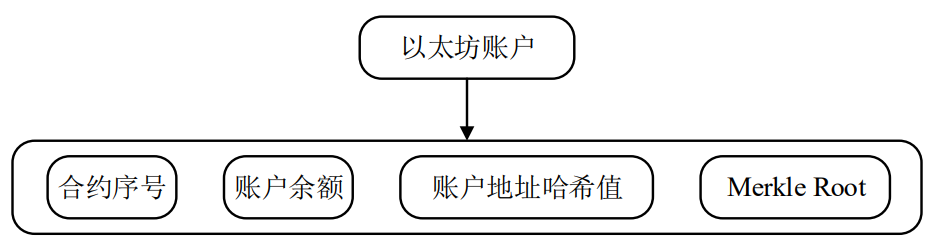
\includegraphics[scale=0.6]{ytf}
	\caption{以太坊账户结构模型}
	\label{fig:ytf}
\end{figure}
相对于区块链1.0和区块链2.0,区块链3.0并没有技术上的提高,也尚无标志性的事件。但区块链3.0对区块链的底层技术和性能作出了更高的要求,以实现更大规模的应用。\par
\subsubsection{比特币与法律规制}
之前在我们小组的汇报演讲中就提到了比特币常常被用于非法交易,正因为此种犯罪交易所得高且不易被侦破,犯罪分子便更加肆无忌惮,越来越多的人走上了这种不归路。这也说明比特币交易的去中心化、隐秘性、虚拟性、流通自由性等特征会给社会乃至世界带来一些消极影响。比特币现在还处在其发展的初级阶段,它的产生和发展给传统货币体系带来了颠覆性的影响,急需建立完善的监管制度防范其风险。比特币对个人、社会、法律发出了三重挑战,作为学习计算科学的大学生,我们应该做到理性地面对这些挑战。\par
\subsubsection{区块链面临的问题}
一是存储空间的相对稀缺性。目前,比特币的钱包已经需要占用几百G的存储空间,一般的手机都无法使用,普通台式机也够呛,进行一次比特币转账,根本没法实时到账,须长时间对大量进行存储才能完成。\par
二是安全的相对有效性。区块链技术是防篡改、匿名的,但是,如果是区块链的主导者,是否可以篡改区块链的相关数据呢?正是因为这样的疑问,一些人认为区块链的防骗是相对的。比如,比特币持有者就出现过被盗的情况。试想,如果盗贼没有技术篡改能力,那如何盗取别人的比特币?很多技术都有缺陷都有漏洞,尤其是互联网通信技术和计算机技术,他们需要经常弥补这些漏洞,但也无法保证这些技术完美无缺\citep{huangqifan}。\par
\subsection{比特币的“去中心化”}
区块链的作用机制通过分布式的对等网络实现。这一属性与经常用来形容区块链的去中心化(decentralized)相联系。区块链的这一属性强调了区块链的技术特点,尤其是公有链——它无需一个中心服务器,由散布在世界各地的、愿意加入的节点来构建区块链。\par
那这种“去中心化”真的使区块链没有中心么?第一,在区块链中,只要每个人都记录所有人数据,那每个人都可能成为一个中心,所以有人认为区块链不是“去中心化”,而是“多中心化”;第二,区块链中一定有“群主”,这个群主是不是中心?第三,区块链中的规则由谁制定?规则可不可以修改?制定和修改规则的人是不是中心?或许区块链的“去中心化”很可能是在“去化别人的、传统的中心,而确立自己为中心”\citep{huangqifan}。\par
\subsection{比特币的未来发展}
通过对“A new method to verify Bitcoin bubbles: Based on the production cost”一文的了解,基于现有的资产理论,运用VAR和LPPL模型对基于生产成本的比特币大泡沫进行了验证,通过LPPL模型验证了PECR和BC,下一个比特币大泡沫预计在2020年下半年出现。考虑到比特币将在2020年5月“产量减半”,这一预测是一个高概率事件\citep{jinwuxiong}。\par
区块链技术毕竟尚处于早期萌发阶段,其理论基础、应用场景、技术安全、标准监管等还要大量完善。第一,未来制度的完善是发挥区块链技术优势的必要保证。正规制度包括法律法规、行业标准是区块链发展的必要条件。如果出现买方拒绝付款或者卖方拒绝提供商品等行为,则需要法律法规的补充与完善,最好还能再通过征信平台对名誉的价值进行管制。第二,未来区块链对信息产权的明晰将提出更高的要求。这与现在的信息时代面临相同的问题,数据产权的界定不清将会限制数据资源的使用与正常交易。因此,如果想要发挥区块链在信息共享中的作用,对信息的归属与如何使用需要进一步的完善\citep{liuyanghe}。\par
\section{总结}
时光荏苒,大一的第一个学期就这么即将逝去。这学期跟随孙教授学习计算科学,让我对计算机系统网络有了一个清楚且较为完整的认识。分组演讲环节也让我对区块链与比特币有了一定了解,我相信这些知识定能成为我日后学习计算机的垫脚石。我认为区块链本身的确是很好的分布式系统,它为人类带来了巨大的方便,但也为我们带来了挑战。很多年轻人怀揣着一夜暴富的梦想投身于比特币,的确有人因此得到了财富,但也有人因此倾家荡产。作为学习计算机相关知识的我们,更作为一名大学生,我们应该理性地面对类似比特币这种新型电子货币。全身心地发展自身综合能力与素质才是我们当代大学生应该做的。今后,我将更努力地学习计算机科学,以昂首挺胸的姿态,迎接新知识的挑战。\par
\section{附录}
\begin{itemize}
    \item Github
    个人网址:https://github.com/Silence-upc\par
    \begin{figure}[h!]
    	\centering
    	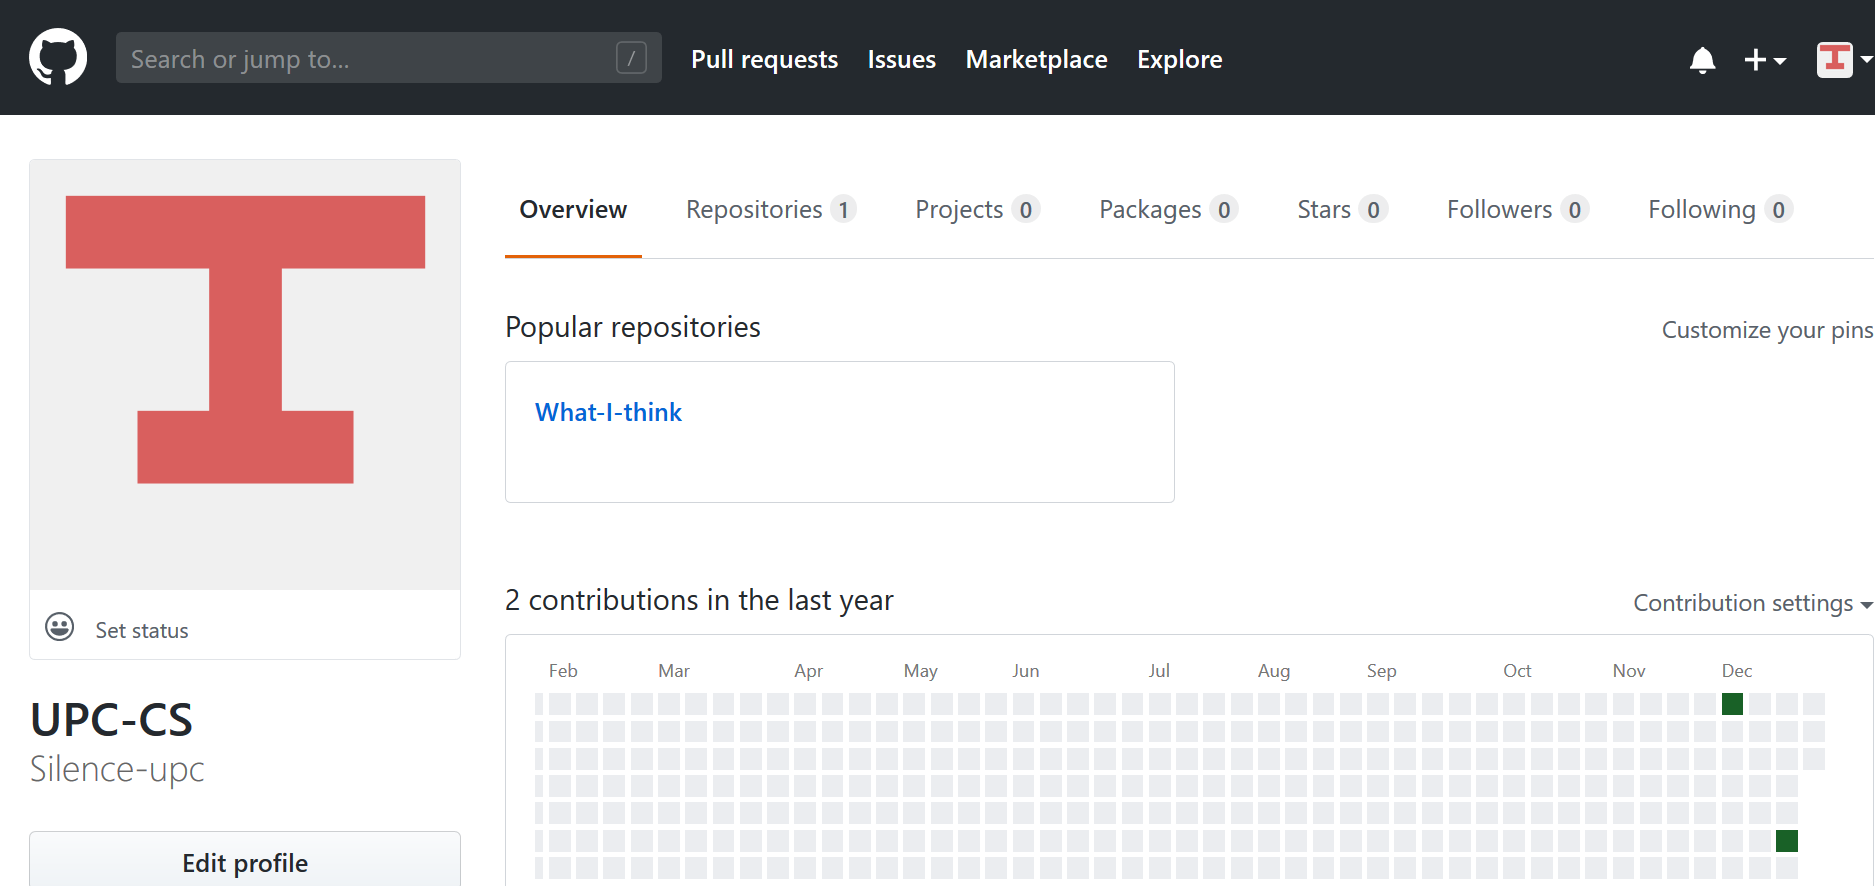
\includegraphics[scale=0.22]{Github}
    	\label{fig:github}
    \end{figure}
    \item 观察者、学习强国、哔哩哔哩APP\par
  \begin{minipage}[t]{0.33\linewidth}
  	\centering
  	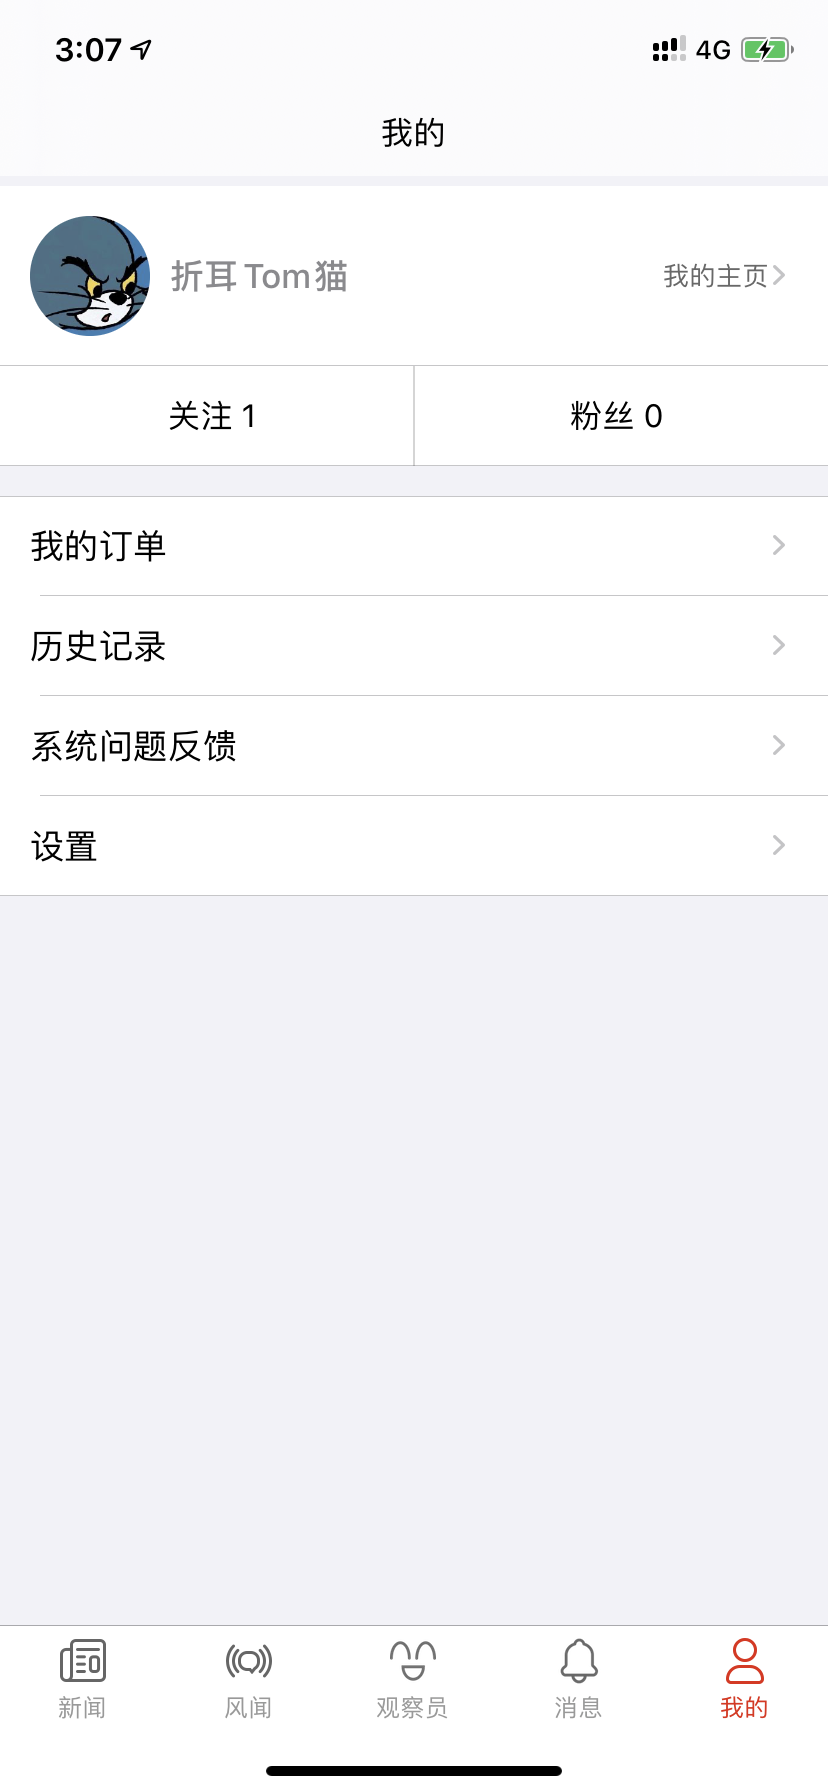
\includegraphics[width=1in]{gcz}
  \end{minipage}
  \begin{minipage}[t]{0.33\linewidth}
	\centering
	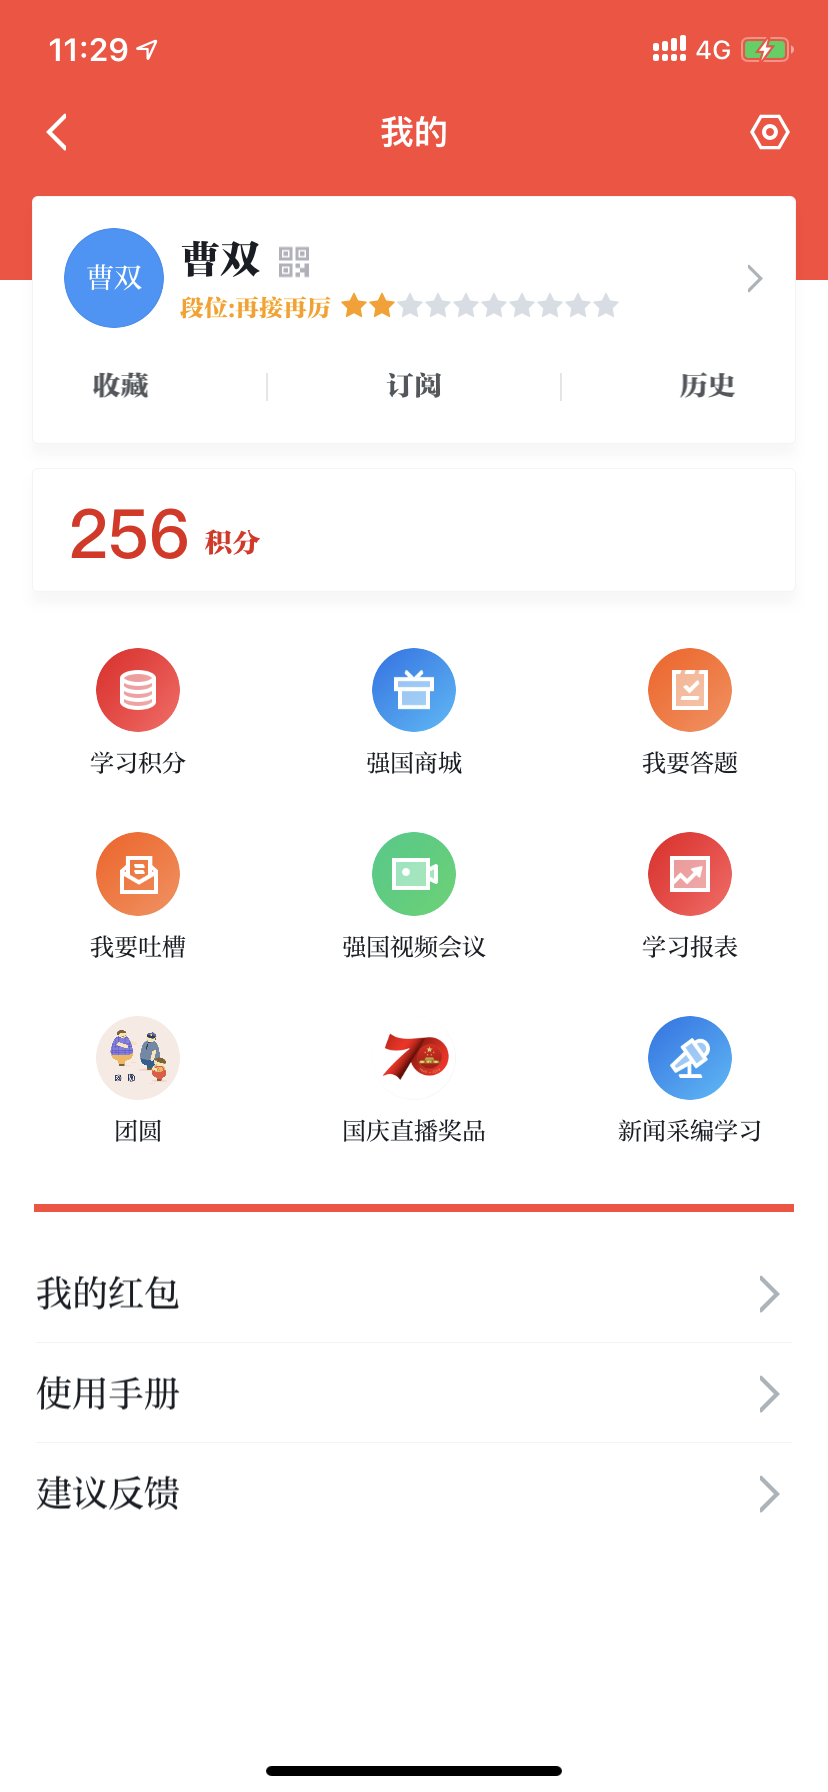
\includegraphics[width=1in]{xxqg}
\end{minipage}
 \begin{minipage}[t]{0.33\linewidth}
	\centering
	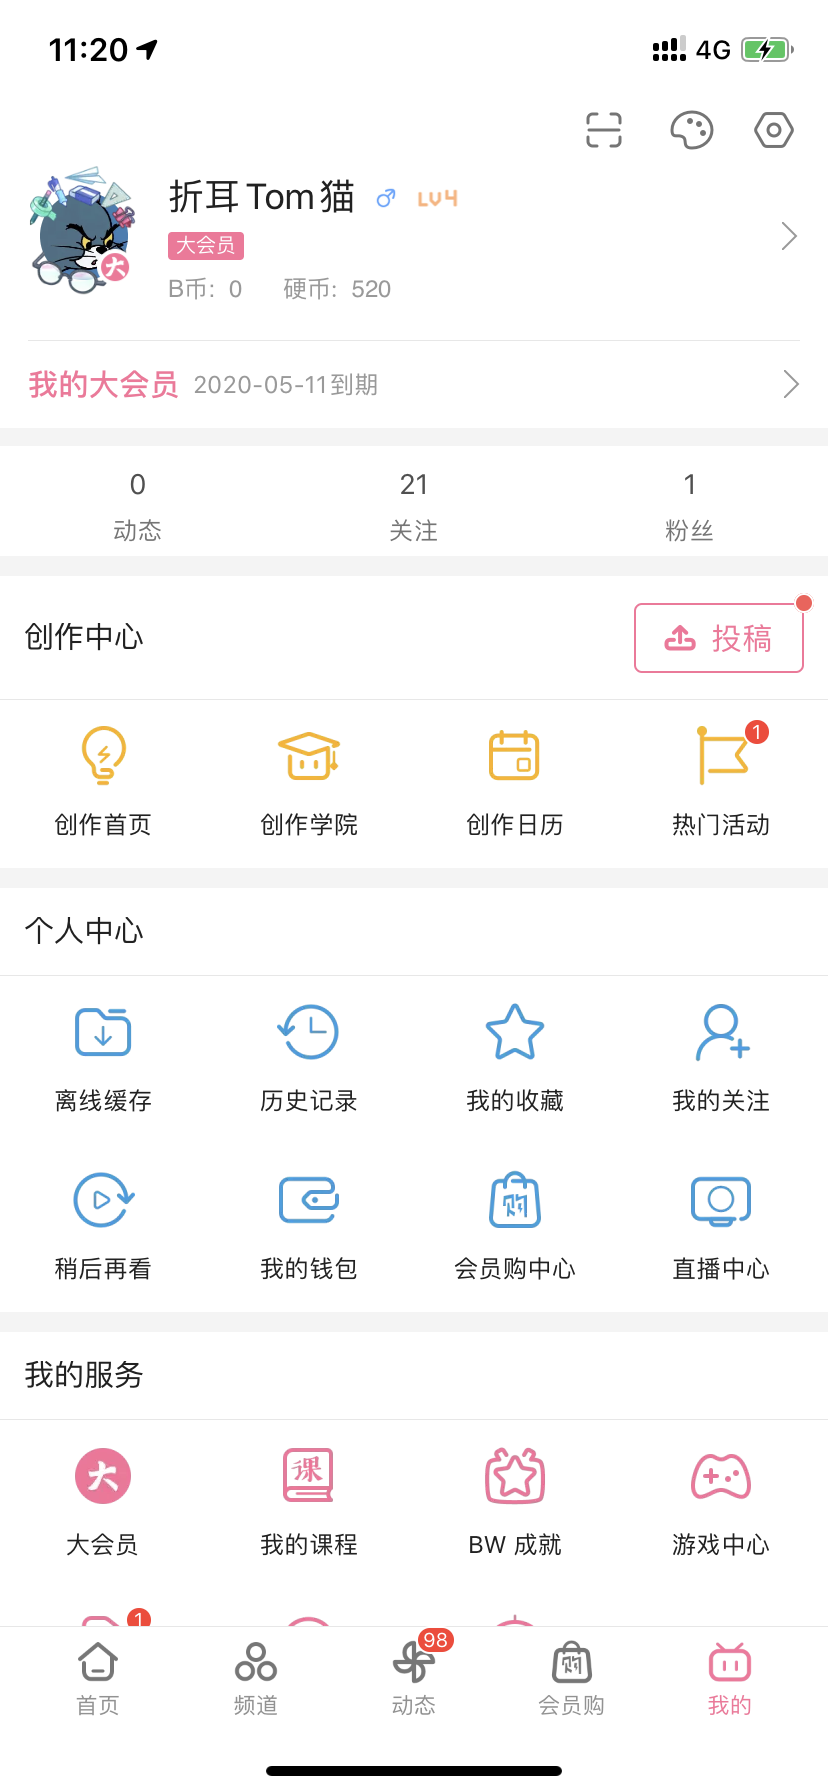
\includegraphics[width=1in]{blbl}
\end{minipage}
    \item CSDN、博客园账户\par
个人网址:https://me.csdn.net/weixin\_45921883\par
   \begin{figure}[h!]
   	\centering
   	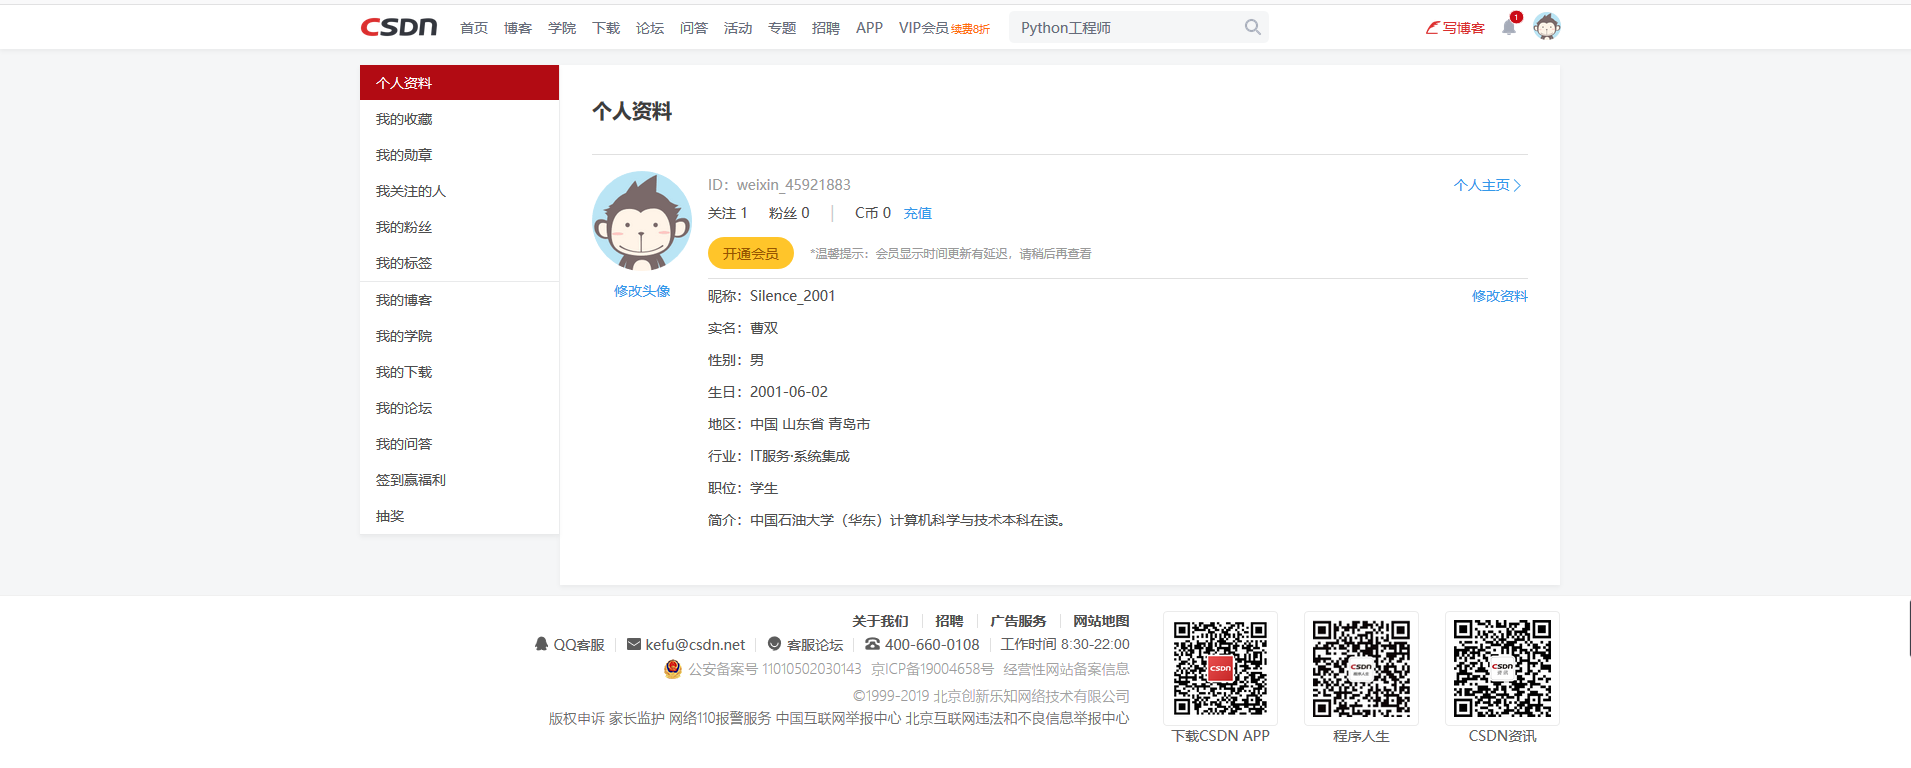
\includegraphics[scale=0.2]{CSDN}
   	\label{fig:CSDN}
   \end{figure}
个人网址:https://home.cnblogs.com/u/1906507/\par
 \begin{figure}[h!]
	\centering
	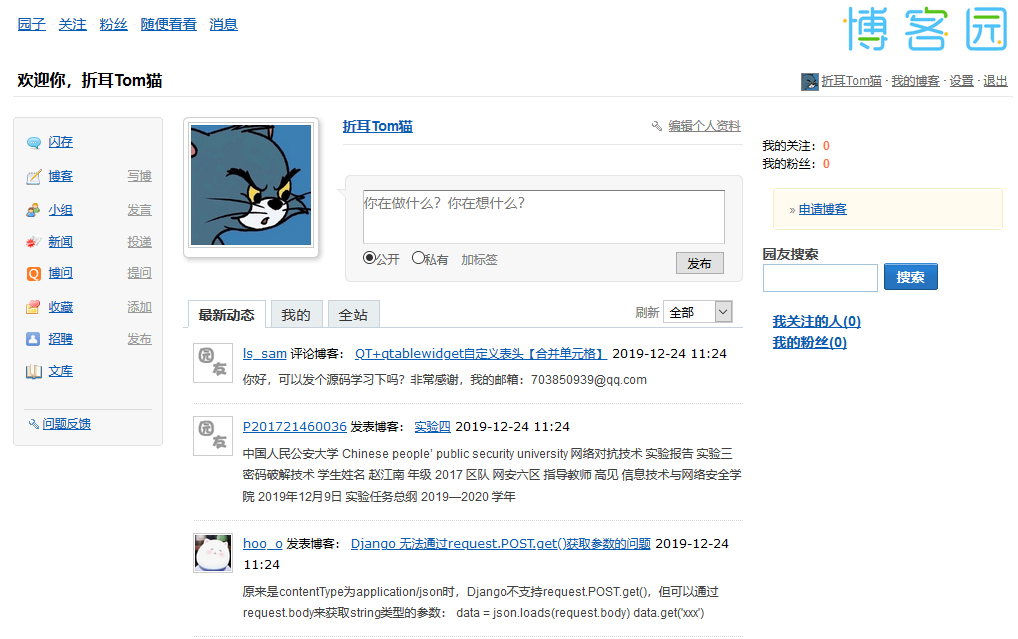
\includegraphics[scale=0.45]{cnblogs}
	\label{fig:cnblogs}
\end{figure}
    \item 小木虫\par
    个人网址:http://muchong.com/bbs/space.php?uid=20208655\par
     \begin{figure}[h!]
    	\centering
    	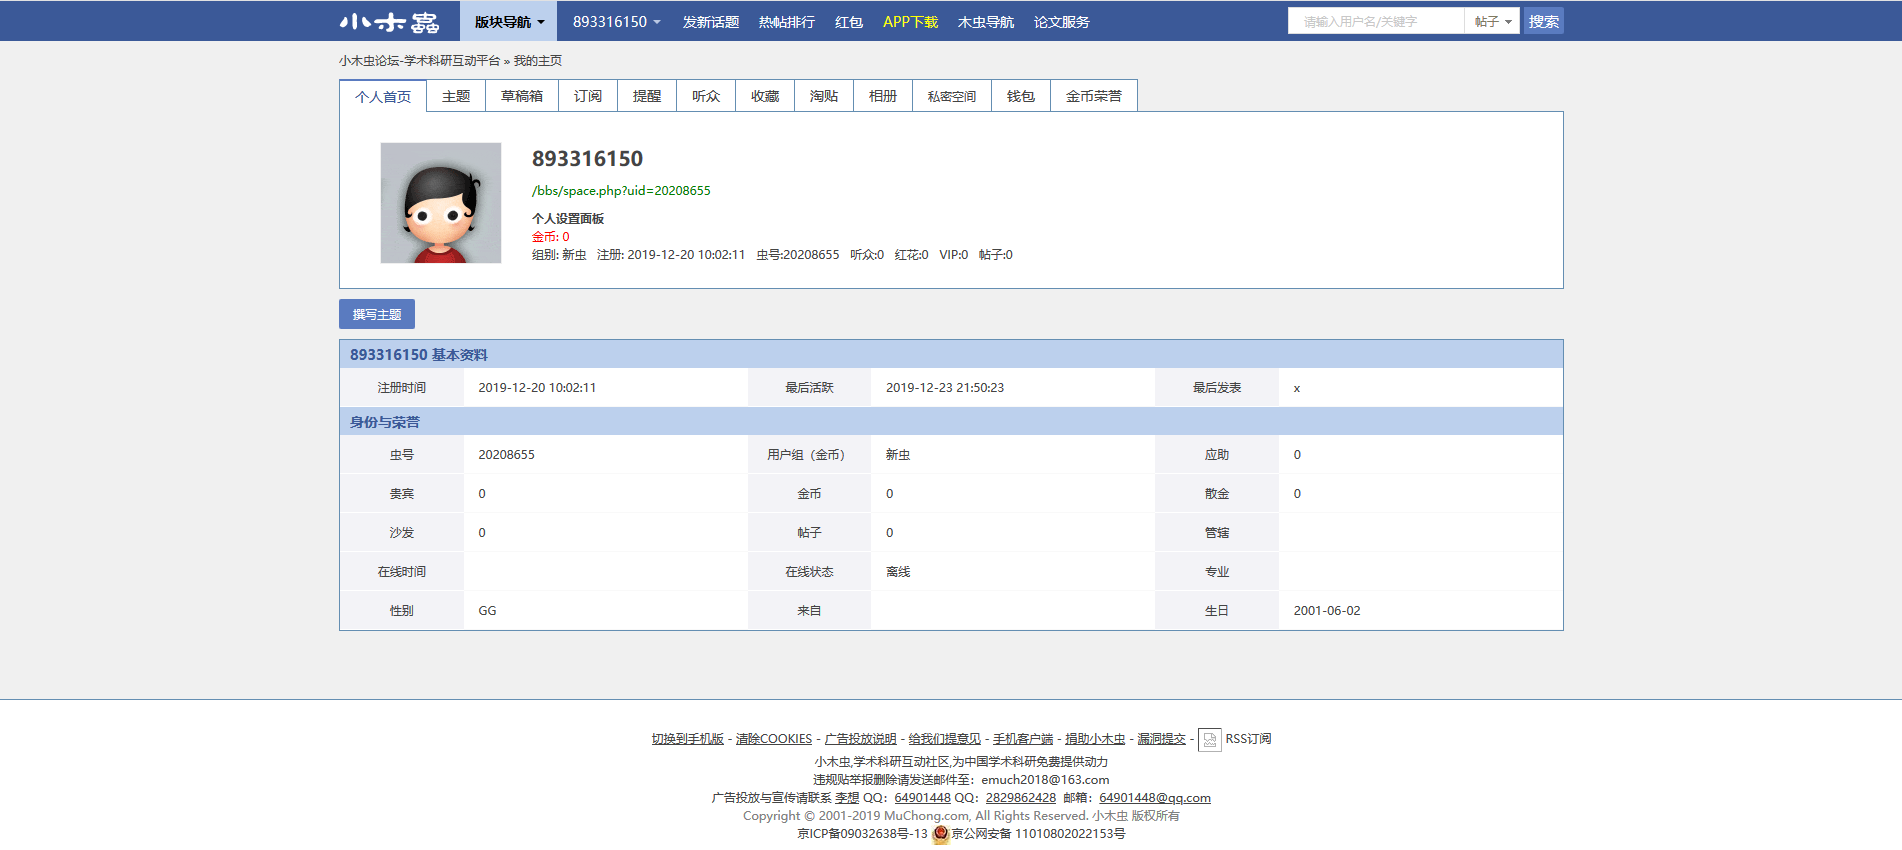
\includegraphics[scale=0.2]{xmc}
    	\label{fig:xmc}
    \end{figure}
\end{itemize}


\hspace*{\fill} \\

\bibliographystyle{plain}
\bibliography{references}


\end{document}
